% use paper, or submit
% use 11 pt (preferred), 12 pt, or 10 pt only

%\documentclass[letterpaper, preprint, paper,11pt]{AAS}	% for preprint proceedings
\documentclass[letterpaper, paper,11pt]{AAS}		% for final proceedings (20-page limit)
%\documentclass[letterpaper, paper,12pt]{AAS}		% for final proceedings (20-page limit)
%\documentclass[letterpaper, paper,10pt]{AAS}		% for final proceedings (20-page limit)
%\documentclass[letterpaper, submit]{AAS}			% to submit to JAS

\usepackage{bm}
\usepackage{amsmath}
\usepackage{subfigure}
\usepackage{float}
%\usepackage[notref,notcite]{showkeys}  % use this to temporarily show labels
\usepackage[colorlinks=true, pdfstartview=FitV, linkcolor=black, citecolor= black, urlcolor= black]{hyperref}
\usepackage{overcite}
\usepackage{footnpag}			      	% make footnote symbols restart on each page




\PaperNumber{16-451}



\begin{document}

\title{MINIMUM ENERGY, REACTION-WHEEL BASED, CUBESAT ATTITUDE CONTROL: A COMPARISON OF COST FUNCTIONS}

\author{Dmitriy Rivkin\thanks{Graduate Student, Department of Computer Engineering, UC Santa Cruz, Santa Cruz, CA, 95064.},  
Qi Gong\thanks{Associate Professor, Department of Applied Mathematics and Statistics, UC Santa Cruz, Santa Cruz, CA, 95064.},
\ and Gabriel Elkaim\thanks{Professor, Department of Computer Engineering, UC Santa Cruz, Santa Cruz, CA, 95064.}
}


\maketitle{} 		


\begin{abstract}
A Legendre pseudospectral method is used to compute energy optimal solutions to a fixed time, large angle satellite attitude maneuver problem using a reaction-wheel based control system. Finding an energy optimal solution is challenging because there are a number of sources of energy usage. Three sources of energy usage are considered: resistive losses (RL), frictional losses (FL), and unrecoverable mechanical (UM) energy. To handle non-smoothness of the UM cost function efficiently, a smooth approximation of the UM cost is introduced. "Bang-Off-Bang" type solutions, maneuvers consisting of an impulsive kick, a zero-energy coast, and a second impulsive kick to arrest motion at the desired location, are found to optimize both FL and UM costs. RL costs are minimized by a different, smooth, solution.
\end{abstract}


\section{Introduction}
CubeSats, small satellites in the form of a 10cm cube, operate under severe energy constraints, their only source of energy being a batteries which are recharged by solar panels covering the (very small) body. High performance attitude controllers can increase the capabilities of these small spacecraft, but unfortunately consume a significant fraction of the energy budget. As such, it is valuable to minimize the energy cost of attitude maneuvers. This work uses a pseudospectral optimal control method to compute energy optimal, large angle slew trajectories for a 1U CubeSat using a reaction-wheel based attitude controller. 

\section{Hardware Background}
Reaction-wheel attitude control is based on the principle of momentum exchange between the wheels and the satellite body. When a torque is exerted on a reaction wheel by a motor (usually a brushless DC [BLDC] motor), the opposite torque is exerted on the satellite body. Three reaction wheels, arranged orthogonally, allow for control in three axes. This is a popular attitude control method because it does not consume any fuel, using electrical energy from batteries which can be regenerated by solar panels. Other methods of electrical energy attitude control include electro-magnetic torquers, but these tend to impart very small forces on the satellite.\\


\section{Problem Description}
This work is concerned with the computation of a control trajectory for a large angle slew maneuver which minimizes the total electrical energy consumed by the BLDC motors that provide actuation torque. The torques exerted by the motors on the momentum wheels are the control variables. Three sources of energy consumption are considered:(1) frictional loss, which is proportional to wheel speed squared;(2) resistive loss, which is energy dissipated by armature resistance as the torque-producing current is passed through it, and is proportional to the applied torque squared; (3) energy loss arising when the motor driver is incapable of regenerative braking --- any electrical energy converted into mechanical energy by the motor cannot be converted back into electrical energy, and must be dissipated as heat when the wheel slows down. This energy is denoted as unrecoverable mechanical energy.

\section{Methods}
We use a Legendre pseudospectral method to compute a state-control trajectory pair that minimizes a cost function and satisfies dynamic constraints, as implemented by the software package DIDO\cite{Ross2007}. A similar approach is used by Karpenko \cite{Karpenko2014} for time optimal reorientation, and Lee \cite{Lee2014} uses a pseudospectral method to optimize for time and energy simultaneously, in the presence of restricted zones. The Lee paper defines an energy cost proportional to the magnitude of reaction wheel acceleration, but does not offer a discussion of this choice. This work considers a wider variety of cost functions, and discusses their physical origins. The pseudospectral method produces open loop solutions which can be used as input to a closed loop controller. A practical implementation of an optimal trajectory tracking algorithm is described by Karpenko \cite{Karpenko2014}.


\section{Optimal Control Problem Formulation}

The optimal control problem is formulated as follows (refer to Table \ref{tab:notation} for notation):

\begin{align*}
	\text{Minimize cost functional } \;\;\; J \\ 
	\text{Subject to}: \;\;\; \mathbf{\dot{x}} = \textbf{f}(\textbf{x},\textbf{u}) \\
	\mathbf{x}(t_{0}) = \mathbf{x_{0}}\\
	\mathbf{x}(t_{f}) = \mathbf{x_{f}}\\
	\mathbf{u_{L}} \leq \mathbf{u} \leq \mathbf{u_{U}} 	\\
	\mathbf{x_{L}} \leq \mathbf{x} \leq \mathbf{x_{U}} \\
	t_{0}\text{ and } t_{f} \text{ fixed}
\end{align*}

where the dynamic constraints, $\textbf{f}(\textbf{x},\textbf{u})$, are, as derived by Karpenko \cite{Karpenko2014}: 


\begin{align*}
\begin{bmatrix}
\dot{\pmb{\omega}}\\
\dot{\pmb{\omega}_{w}}
\end{bmatrix} = \pmb{\Gamma}^{-1} 
\begin{bmatrix}
-\pmb{\omega} \times ( \pmb{I\omega}+\sum_{i=1}^{3}\pmb{a}_{i}I_{w,i}\pmb{\omega}_{w,i} +\pmb{a}_{i}I_{w,i}\pmb{a}_{i}^{T}\pmb{\omega})\\
\pmb{u}
\end{bmatrix}\\
\pmb{\Gamma} = 
\begin{bmatrix}
\pmb{I}+\sum_{i=1}^{3}\pmb{a}_{i}I_{w,i}\pmb{a}_{i}^{T} & \pmb{a}_{1}I_{w,1} & \pmb{a}_{2}I_{w,2} & \pmb{a}_{3}I_{w,3}\\
I_{w,1}\pmb{a}_{1}^{T} & I_{w,1} & 0 & 0\\
I_{w,2}\pmb{a}_{2}^{T} & 0 & I_{w,2} & 0\\
I_{w,3}\pmb{a}_{3}^{T} & 0 & 0 & I_{w,3}
\end{bmatrix}\\
\dot{\pmb{q}} = \frac{1}{2}
\begin{bmatrix}
0 & \pmb{\omega}_{3} & -\pmb{\omega}_{2} & \pmb{\omega}_{1}\\
-\pmb{\omega}_{3} & 0 & \pmb{\omega}_{1} & \pmb{\omega}_{2} \\
\pmb{\omega}_{2} & -\pmb{\omega}_{1} & 0 & \pmb{\omega}_{3} \\
-\pmb{\omega}_{1} & -\pmb{\omega}_{2}& -\pmb{\omega}_{3} & 0 
\end{bmatrix} \pmb{q}
\end{align*}

The cost function $J$ takes on one of the following forms, depending on the optimization being performed.
\begin{align*}
\text{To minimize frictional losses:} \qquad
J = FL = \int_{t_{0}}^{t_{f}} \pmb{\omega}_{w}^{T}\pmb{\omega}_{w} \; dt \\
\\
\text{To minimize resistive losses:} \qquad
J = RL = \int_{t_{0}}^{t_{f}} \pmb{u}^{T}\pmb{u} \; dt \\
\\
\text{To minimize unrecoverable mechanical energy:}\qquad 
J=UM=\int_{t_{0}}^{t_{f}} \sum_{i = 1}^{3}F_{i} \; dt \\
	F_{i}  = \begin{cases}
    \pmb{\omega}_{w,i}\pmb{u}_{i},& \text{if } \pmb{\omega}_{w,i}\pmb{u}_{i}\geq 0\\
    0,              & \text{otherwise}
	\end{cases} \\
\end{align*}




\subsection{Cost Function Practical Considerations}
When performing numerical optimization, it is desirable for the cost function to be continuous and smooth. Cost functions $FL$ and $RL$ satisfy these criteria, while cost function $UM$ is non-smooth at zero. To improve performance, we define an approximate cost function, $\hat{UM}$which is smooth on the interval ($-\infty , +\infty$).

\begin{equation}
\hat{UM} = \int_{t_{0}}^{t_{f}} \sum_{i = 1}^{3}\frac{1}{\alpha}ln(1+e^{\alpha \pmb{\omega}_{w,i} \pmb{u}_{i}}) \; dt, \qquad \alpha > 0 \\
\end{equation}

As the scaling factor, $\alpha$, gets large, $\hat{UM}$ becomes arbitrarily close to $UM$, as illustrated in Figure \ref{f:UMhat}.

\begin{figure}[H]% order of placement preference: here, top, bottom
\centering
 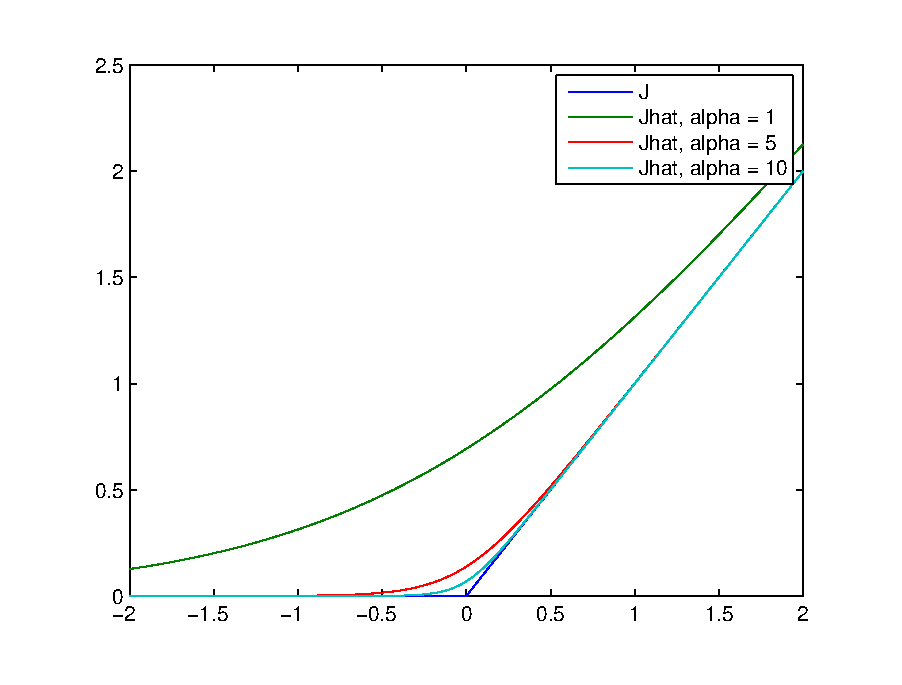
\includegraphics[width = 3in]{cfapprox}
 \caption{$\hat{UM}$ approaches $UM$ as $\alpha$ increases}
 \label{f:UMhat}
\end{figure}

\section{Results}
Control trajectories for a large angle slew of a 1U CubeSat are presented in Figure \ref{f:CT}. The parameters of the satellite and the maneuver can be found in the appendix. Table \ref{tab:pcomp} provides a comparison of the performance of the three numerical solutions with respect to the three cost functions of interest.

\begin{figure}[h]
\centering
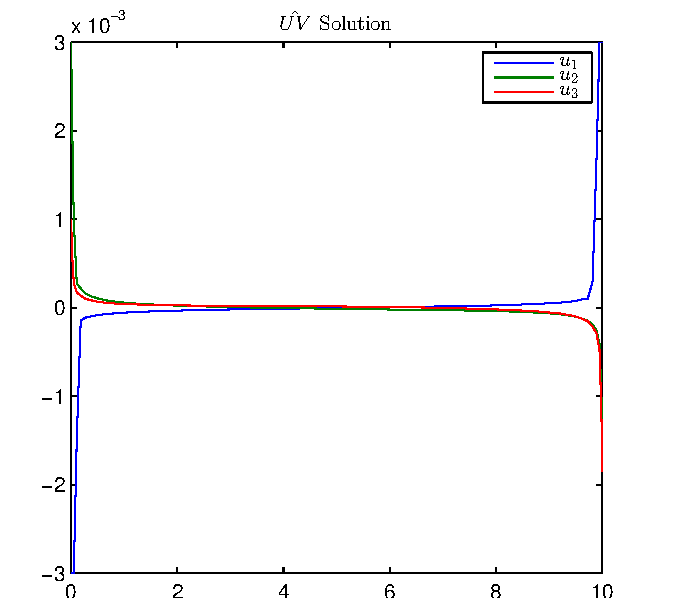
\includegraphics[width = 1.9in]{u_le}
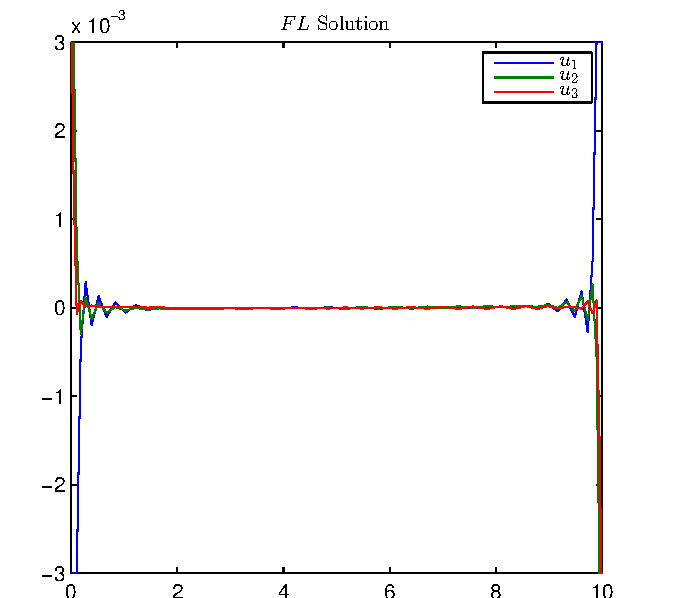
\includegraphics[width = 1.9in]{u_v2}
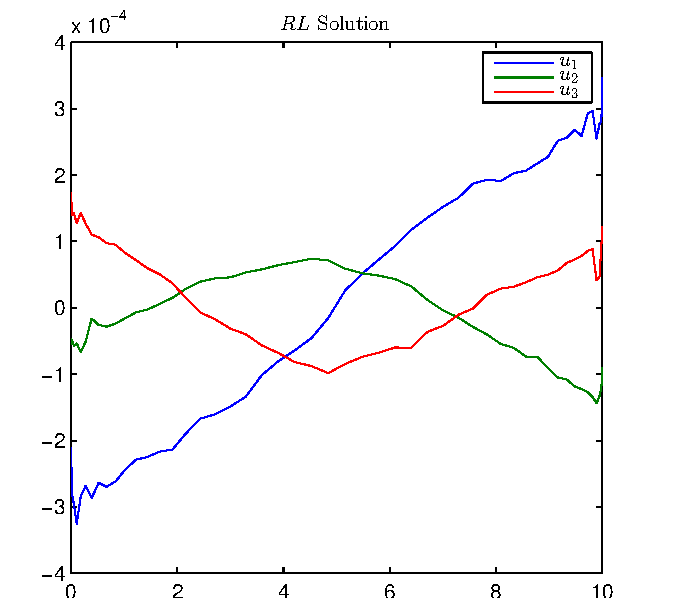
\includegraphics[width = 1.9in]{u_u2}
\caption{Control Trajectories (time (s) vs control torque (Nm))}
\label{f:CT}
\end{figure}

\begin{table}[h]

	\fontsize{10}{10}\selectfont

        \centering 
   \begin{tabular}{c | r | r | r } % Column formatting, 
      \hline 
      Solution    & $UM$ Cost & $FL$ Cost & $RL$ Cost \\
      \hline 
      $\hat{UM}$      & 1.00 & 1.01 & 5.10 \\
      $FL$       & 1.23 & 1.00 & 11.30 \\
      $RL$      & 2.09  & 1.29 & 1.00 \\    
      \hline
   \end{tabular}
   	       \caption{Normalized Performance of Numerical Solutions With Respect to Different Cost Functions}
	   \label{tab:pcomp}
\end{table}
     

\section{Conclusion}
The solutions which optimize cost functions $FL$ and $\hat{UM}$ are the nearly the same and have Bang-Off-Bang form. However, they both incur a high RL cost. On the other hand, the control which optimizes $RL$ is continuous, which can be desirable from the point of view of numerical optimization. It also performs reasonably well with respect to $FL$. However, it performs poorly with respect to $UM$, indicating that optimizing with respect to any one of these three cost functions does not yield a truly optimal solution. A better approach would be to optimize a cost function which is a weighted sum of the three, the relative weights being dependent on the specific system at hand. 

\section{Notation}
\begin{table}[h!]
	\fontsize{10}{10}\selectfont
    \caption{Notation}
   \label{tab:notation}
        \centering 
   \begin{tabular}{c r } % Column formatting, 
      \hline 
      $\mathbf{u}$ & Column vector of the torques exerted by the motors  \\
      $\pmb{\omega}_{w}$      & Column vector of reaction wheel speeds W.R.T satellite body \\
      $\pmb{\omega}$       & Body frame angular velocity W.R.T inertial frame, in body coordinates \\
      $\pmb{q}$      & Unit quaternion expressing body frame attitude \\
      $\pmb{x}$ & $\lbrack 
      \pmb{\omega}^T \;\pmb{\omega}_{w}^{T} \; \pmb{q}^{T}
      \rbrack^{T}$\\
      $\pmb{a}_{i}$ & Orientation of spin axis of wheel $i$ w.r.t body frame \\
      $\pmb{I}$ & Inertia tensor of spacecraft with freely rotating wheels \\
      $I_{w,i}$ & Moment of inertia of wheel $i$ about its spin axis \\
      \hline
   \end{tabular}
\end{table}

\section{Appendix: Values used for Optimization}
\begin{align*}
t_{0} = 0 \; s \\
t_{f} = 10 \; s \\
\lbrack yaw, pitch, roll\rbrack_{0} = \lbrack 0, 0, 0\rbrack rad \\
\lbrack yaw, pitch, roll\rbrack_{f} = \lbrack -\frac{\pi}{3}, \frac{\pi}{5}, \pi \rbrack \; rad \\
\pmb{u}_{L} = -\pmb{u}_{U} = \begin{bmatrix}3 & 3 & 3 \end{bmatrix}^{T} \times 10^{-3} \; Nm \\
\pmb{\omega}_{w,L} = -\pmb{\omega}_{w,U} = \begin{bmatrix} 600 & 600& 600 \end{bmatrix}^{T} \; rad/s \\
I_{w,1} = I_{w,2} = I_{w,3} = 1.01 \times 10^{-4} \; kg. m^{2} \\
\pmb{I} = \begin{bmatrix}
153 & 2 & 2 \\
2 & 153 & 2 \\
2 & 2 & 153
\end{bmatrix} \times 10^{-5} \; kg. m^{2}\\
\pmb{a}_1 = \begin{bmatrix}
1 \\ 0 \\ 0
\end{bmatrix} \; , \;
\pmb{a}_2 = \begin{bmatrix}
0 \\ 1 \\ 0
\end{bmatrix} \; , \;
\pmb{a}_3 = \begin{bmatrix}
0 \\ 0 \\ 1
\end{bmatrix} \;\\
\end{align*}


\bibliographystyle{AAS_publication}   % Number the references.
\bibliography{C:/Users/Dmitriy/Documents/library}   % Use references.bib to resolve the labels.



\end{document}
